\newpage
\begin{appendices}
    \section{Raw and Processed Data for B and E Strings}
        \begin{figure}[!htbp]
            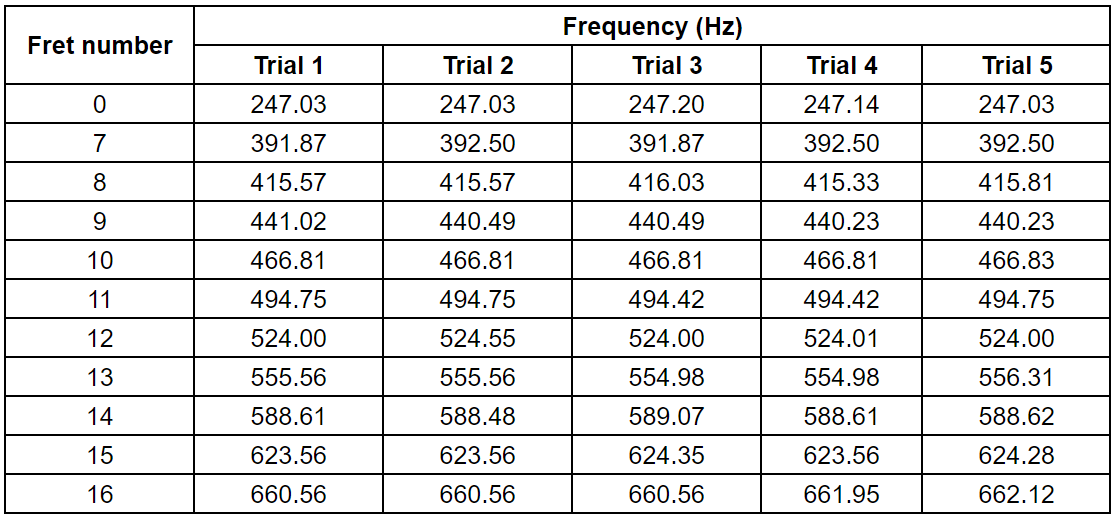
\includegraphics[width = \textwidth]{ee/b string raw.png}
            \caption{Raw data for B string}
        \end{figure}
        \begin{figure}[!htbp]
            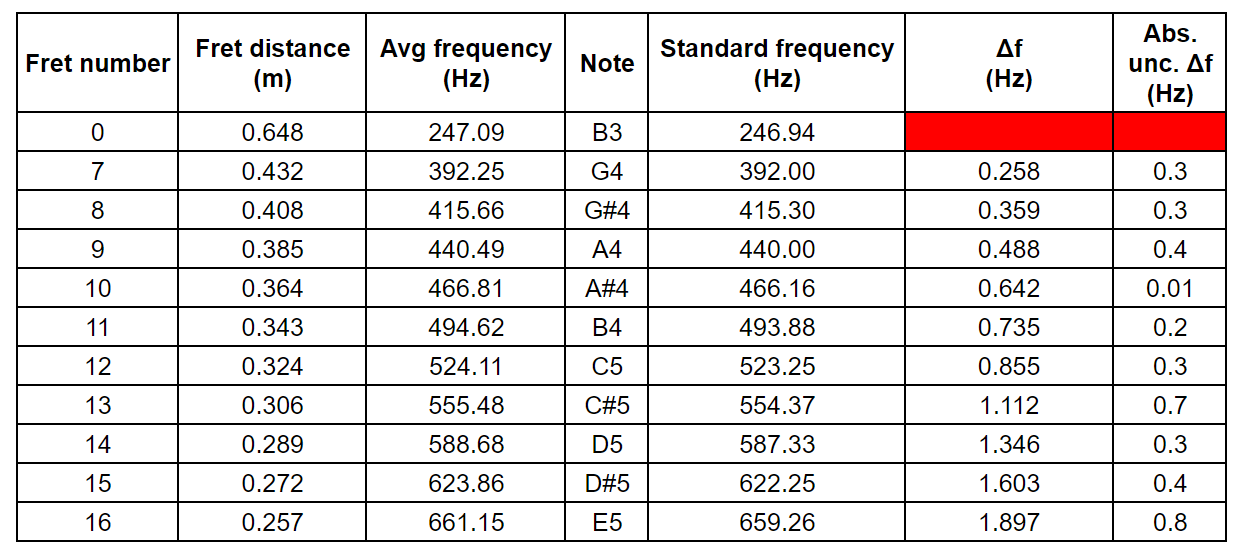
\includegraphics[width = \textwidth]{ee/b string prsd.png}
            \caption{Processed data for B string}
        \end{figure}
        \begin{figure}[!htbp]
            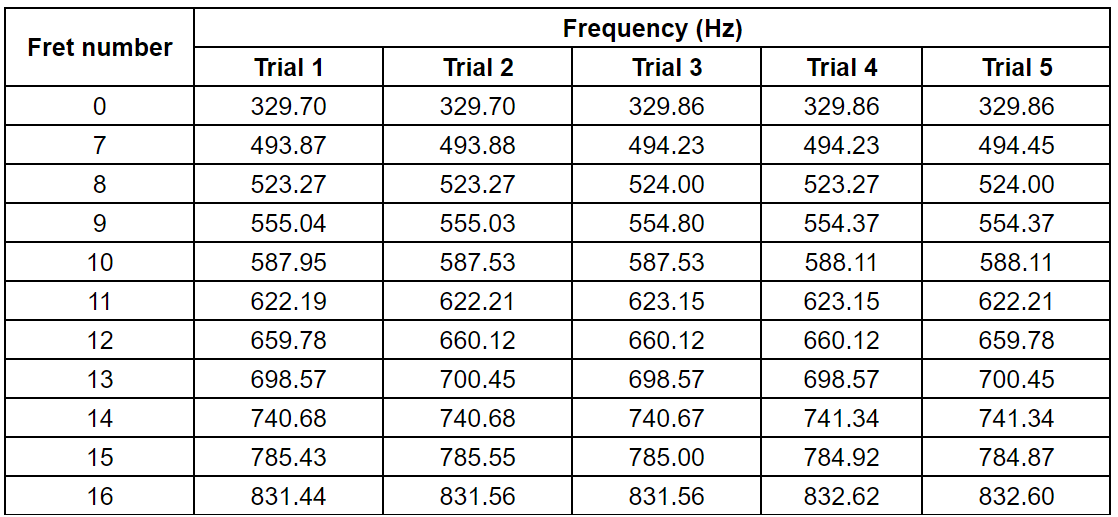
\includegraphics[width = \textwidth]{ee/e string raw.png}
            \caption{Raw data for E string}
        \end{figure}
        \begin{figure}[!htbp]
            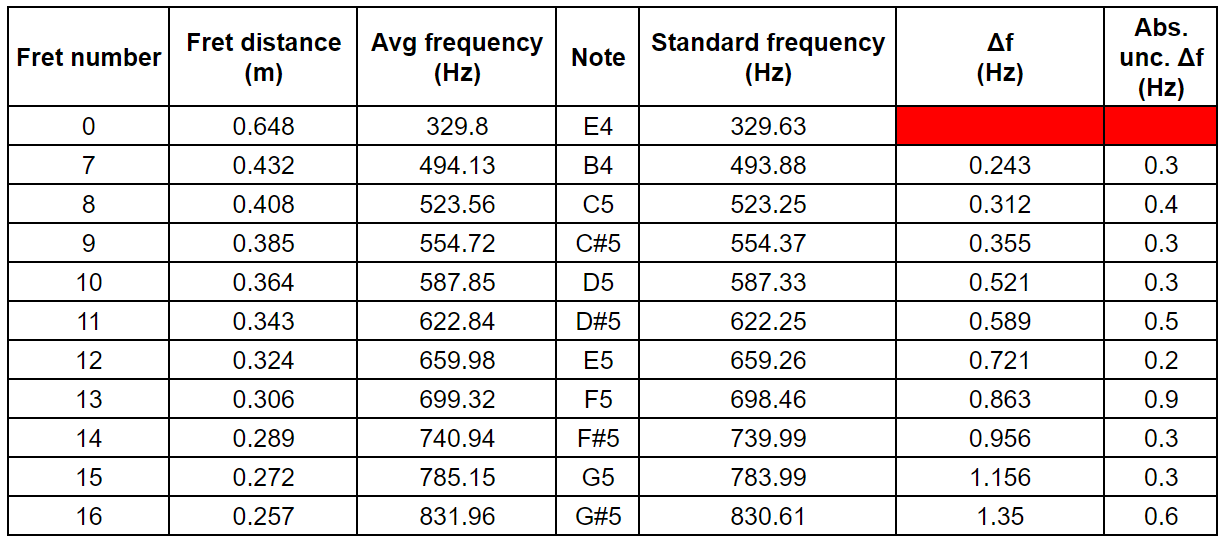
\includegraphics[width = \textwidth]{ee/e string prsd.png}
            \caption{Processed data for E string}
        \end{figure}
\end{appendices}
